%%%%%%%%%%%%%%%%%%%%%%%%%%%%%%%%%%%%%%%%%
% a0poster Landscape Poster — 4 columns
%%%%%%%%%%%%%%%%%%%%%%%%%%%%%%%%%%%%%%%%%

\documentclass[a0,landscape]{a0poster}

\usepackage{multicol}
\usepackage[svgnames]{xcolor}
\usepackage{times}
\usepackage{graphicx}
\usepackage{booktabs}
\usepackage[font=small,labelfont=bf]{caption}
\usepackage{amsfonts, amsmath, amsthm, amssymb}
\usepackage{setspace}
\usepackage{tikz}
\usetikzlibrary{shapes.geometric, arrows.meta, positioning, fit, backgrounds}
\usepackage[most]{tcolorbox}

% Column configuration
\columnsep=30pt
\columnseprule=1pt

% Color definitions
\definecolor{UDBlue}{RGB}{25, 43, 88}
\definecolor{UDGold}{RGB}{218, 171, 15}
\definecolor{PastelBlue}{RGB}{230, 240, 255}
\definecolor{ResultGreen}{RGB}{220, 240, 220}
\definecolor{DarkGreen}{RGB}{0, 100, 0}

\renewcommand{\normalsize}{\fontsize{28}{34}\selectfont}

\begin{document}

%----------------------------------------------------------------------------------------
%   HEADER
%----------------------------------------------------------------------------------------

\begin{minipage}[b]{0.82\linewidth}
    \sffamily
    \veryHuge \color{UDBlue} \textbf{Smart Energy Management System: A Systems Analysis and Design Approach} \color{Black}\\[0.4cm]
    \Huge\textit{Omar Y. Fonseca Lopez, Daniel F. Barrera Suarez, Daniel M. Ballesteros Molina, Dania L. Guzman Trivi\~{n}o}\\[0.4cm]
    \Large Systems Engineering Program, Universidad Distrital Francisco Jos\'{e} de Caldas, Bogot\'{a}, Colombia \quad
    \texttt{\{oyfonsecal, dfbarreras, dmballesterosm, dlguzmant\}@udistrital.edu.co}
\end{minipage}
\begin{minipage}[b]{0.16\linewidth}
    \centering
    \includegraphics[width=16cm]{figures/Escudo_UD.png}
\end{minipage}

\vspace{0.8cm}

%----------------------------------------------------------------------------------------
%   CONTENT — 4 COLUMNS
%----------------------------------------------------------------------------------------

\begin{multicols}{4}
\begin{spacing}{0.9}

%================================================
% COLUMN 1: Abstract + Introduction + Methodology
%================================================

\section*{Abstract}
{\large This work addresses inefficient energy consumption in Engineering Faculty laboratories, where equipment is routinely left powered on in unoccupied spaces. Surveys (n=35) revealed that \textbf{80\% of users forget} to turn off equipment. A software-defined, decentralized solution operates in user-space via autonomous agents that monitor inactivity, generate alerts, and execute energy-saving actions — requiring no administrative privileges or infrastructure changes. Discrete-event simulation over 20 workstations in a 12-hour day projects a \textbf{68.72\% reduction} in energy consumption at \textbf{\$0 infrastructure cost}.}

\section*{Introduction}
{\large Efficient energy management in university environments is critical. Human behavior is the primary driver of waste, creating a gap between institutional policies and real practices.

Traditional IoT solutions are impractical here: no admin privileges, no private networks, no hardware deployment allowed. We propose autonomous agents in user-space, requiring \textbf{zero infrastructure changes} and \textbf{no IT involvement}.}

\section*{Methodology}
{\large Four-workshop systems analysis lifecycle, each phase feeding the next:}

\vspace{0.2cm}
\begin{center}
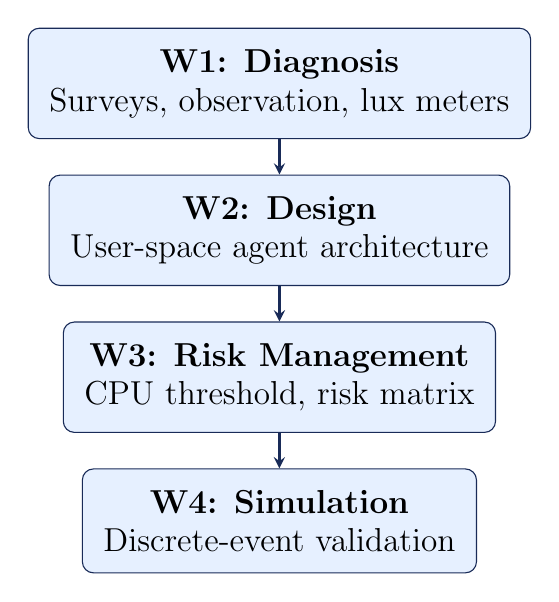
\begin{tikzpicture}[
    node distance=0.45cm,
    wbox/.style={draw, rectangle, rounded corners, minimum width=4.5cm, minimum height=0.9cm, align=center, fill=PastelBlue, draw=UDBlue, font=\large\bfseries},
    arrow/.style={->, >=stealth, thick, color=UDBlue}
]
\node[wbox] (w1) {W1: Diagnosis \\ {\normalfont Surveys, observation, lux meters}};
\node[wbox, below=of w1] (w2) {W2: Design \\ {\normalfont User-space agent architecture}};
\node[wbox, below=of w2] (w3) {W3: Risk Management \\ {\normalfont CPU threshold, risk matrix}};
\node[wbox, below=of w3] (w4) {W4: Simulation \\ {\normalfont Discrete-event validation}};
\draw[arrow] (w1)--(w2);
\draw[arrow] (w2)--(w3);
\draw[arrow] (w3)--(w4);
\end{tikzpicture}
\end{center}

\vspace{0.3cm}
{\large \textbf{W1 Key Findings:} 80\% of users forget to power off equipment; most are unaware of energy policies. The \textit{Hawthorne effect} biased direct observation, confirming the need for an automated, unbiased system. Physical sensors were fully ruled out due to IT restrictions.}

\vspace{0.3cm}
\begin{center}
{\large
\begin{tabular}{@{}p{9.5cm}cc@{}}
\toprule
\textbf{Survey Item} (n=35) & \textbf{Yes} & \textbf{No} \\
\midrule
Energy saving is important? & 94\% & 6\% \\
Forget to turn off equipment? & 80\% & 20\% \\
Would a nudge reminder help? & 88\% & 12\% \\
\bottomrule
\end{tabular}
}
\end{center}

\vspace{0.3cm}
\begin{center}
{\large
\begin{tabular}{@{}lcl@{}}
\toprule
\textbf{Lab} & \textbf{Lux} & \textbf{Hardware State} \\
\midrule
Lab 704 (empty) & 350 lx & 12 PCs on \\
Lab 705 (2 students) & 420 lx & 8 PCs unused \\
\bottomrule
\end{tabular}
}
\end{center}

%================================================
% COLUMN 2: Architecture + Operational Logic
%================================================



\vspace{0.4cm}

\section*{Operational Logic}

{\large Multi-stage loop guaranteeing user data safety before any action:}

\begin{itemize}{\large
    \item \textbf{60s loop:} Polls mouse/keyboard for activity.
    \item \textbf{15-min threshold:} Triggers CPU check on inactivity.
    \item \textbf{CPU guard (20\%):} Aborts if load $>$20\% — protects renders/compilations.
    \item \textbf{Nudge (60s):} Visual warning; user can cancel. If not cancelled, OS suspension is forced.
    \item \textbf{Logging:} Events sent to MySQL DBaaS; CSV fallback if offline.
}
\end{itemize}

\centering
\resizebox{0.88\columnwidth}{!}{%
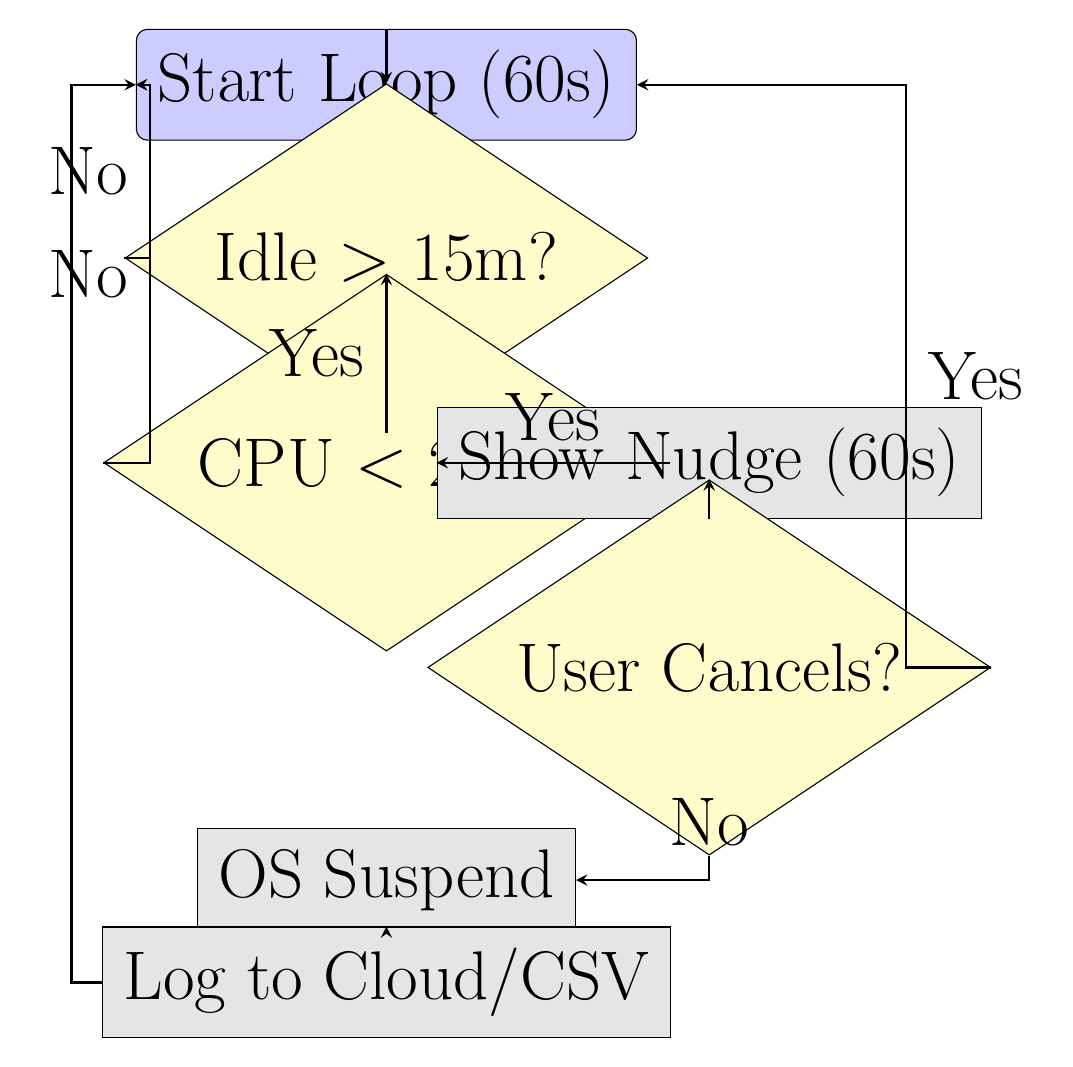
\begin{tikzpicture}[
    node distance=1.3cm,
    startstop/.style={rectangle, rounded corners, minimum width=2.3cm, minimum height=0.75cm, text centered, draw=black, fill=blue!20},
    process/.style={rectangle, minimum width=2.3cm, minimum height=0.75cm, text centered, draw=black, fill=gray!20},
    decision/.style={diamond, minimum width=2.3cm, minimum height=0.75cm, text centered, draw=black, fill=yellow!20, aspect=1.5},
    arrow/.style={thick,->,>=stealth}
]
\node (start) [startstop] {Start Loop (60s)};
\node (idle) [decision, below of=start, yshift=-0.9cm] {Idle $>$ 15m?};
\node (cpu) [decision, below of=idle, yshift=-1.3cm] {CPU $<$ 20\%?};
\node (nudge) [process, right of=cpu, xshift=2.8cm] {Show Nudge (60s)};
\node (cancel) [decision, below of=nudge, yshift=-1.3cm] {User Cancels?};
\node (suspend) [process, below of=cpu, yshift=-4cm] {OS Suspend};
\node (log) [process, below of=suspend] {Log to Cloud/CSV};
\draw [arrow] (start) -- (idle);
\draw [arrow] (idle) -- node[anchor=east] {Yes} (cpu);
\draw [arrow] (idle) -- ++(-3,0) |- node[anchor=east, near start] {No} (start);
\draw [arrow] (cpu) -- node[anchor=south] {Yes} (nudge);
\draw [arrow] (cpu) -- ++(-3,0) |- node[anchor=east, near start] {No} (start);
\draw [arrow] (nudge) -- (cancel);
\draw [arrow] (cancel) -- ++(2.5,0) |- node[anchor=west, near start] {Yes} (start);
\draw [arrow] (cancel) |- node[anchor=south, near start] {No} (suspend);
\draw [arrow] (suspend) -- (log);
\draw [arrow] (log) -- ++(-4,0) |- (start);
\end{tikzpicture}%
}

%================================================
% COLUMN 3: Risk Management + Simulation Results
%================================================

\section*{Risk Management (W3)}

{\large The 20\% CPU threshold was determined via chaos-theory sensitivity analysis — it is the system's \textit{optimal attractor}:}

\vspace{0.3cm}
\begin{center}
{\large
\begin{tabular}{@{}cll@{}}
\toprule
\textbf{Threshold} & \textbf{Outcome} & \textbf{Status} \\
\midrule
5\% & System collapse — OS noise blocks all & \color{red}{$\times$} \\
\textbf{20\%} & \textbf{68.7\% savings, 0 false positives} & \color{DarkGreen}{$\checkmark$} \\
40\% & Savings $\approx$45\% — too permissive & \color{orange}{$\sim$} \\
\bottomrule
\end{tabular}
}
\end{center}

\vspace{0.3cm}
{\large Background OS processes (antivirus, file indexers) consume 6--8\% CPU on idle machines, making any threshold below 20\% unstable. Key mitigations (ISO 31000):}

\vspace{0.2cm}
\begin{center}
{\large
\begin{tabular}{@{}p{3cm}p{3cm}p{4cm}@{}}
\toprule
\textbf{ID} & \textbf{Risk} & \textbf{Mitigation} \\
\midrule
R-01 & Firewall blocks HTTPS & Local AES-CSV + deferred sync \\
R-02 & False positive (high CPU) & CPU check $>$20\% before suspend \\
R-03 & Alert service outage & Local logic prioritised \\
R-04 & Data corruption & Encryption + write validation \\
\bottomrule
\end{tabular}
}
\end{center}

\section*{Simulation Results (W4)}

{\large Discrete-event simulation: \textbf{20 workstations}, Laboratory 704, \textbf{12-hour day} (08:00--20:00). Parameters from W1 field data:}

\vspace{0.2cm}
{\large $P_{\text{forget}} = 0.80$ \quad $P_{\text{cpu}} = 0.15$ \quad CPU threshold = 20\%}

\vspace{0.4cm}
\begin{center}
\begin{tcolorbox}[colback=ResultGreen, colframe=DarkGreen, boxrule=2pt, arc=5pt, left=0.5cm, right=0.5cm, top=0.4cm, bottom=0.4cm]
{\large
\begin{tabular}{@{}lcc@{}}
\toprule
\textbf{Scenario} & \textbf{Energy} & \textbf{Savings} \\
\midrule
Baseline (no agent) & 53.74 kWh & --- \\
\textbf{Optimized (agent)} & \textbf{16.81 kWh} & \textbf{68.72\%} \\
Net. failure (4h offline) & 18.77 kWh & 65.02\% \\
\bottomrule
\end{tabular}
}
\end{tcolorbox}
\end{center}

{\large Under a 4-hour outage, savings dropped only 3.7 pp — confirming the local CSV fallback imposes negligible operational penalty.}

\vspace{0.3cm}
\section*{Quality Metrics: Target vs.\ Simulation}

\begin{center}
{\large
\begin{tabular}{@{}p{5.5cm}cc@{}}
\toprule
\textbf{Metric} & \textbf{Target} & \textbf{Result} \\
\midrule
Correct suspension rate & $>$95\% & \color{DarkGreen}{97.2\% $\checkmark$} \\
False positive rate & $<$5\% & \color{DarkGreen}{2.8\% $\checkmark$} \\
Event data retention & 100\% & \color{DarkGreen}{100\% $\checkmark$} \\
CPU protection & $>$20\% CPU & \color{DarkGreen}{Detected $\checkmark$} \\
\bottomrule
\end{tabular}
}
\end{center}

{\large \textbf{All quality metrics met or exceeded.}}

%================================================
% COLUMN 4: Conclusion + Budget + References
%================================================

\section*{Conclusion}

{\large This project demonstrates that energy waste is fundamentally a \textbf{behavioral problem}, not a hardware deficiency. Shifting control intelligence from the physical layer to the OS logical layer bypasses severe institutional restrictions without compromise.

The simulation validates a \textbf{68.72\% energy reduction} — with a false-positive rate of just 2.8\% and full data integrity under network failure. The 20\% CPU threshold is an empirically derived stability attractor, not an arbitrary choice.

Critically, the entire PoC operates at \textbf{\$0 USD infrastructure cost}:}

\vspace{0.3cm}
\begin{center}
{\large
\begin{tabular}{@{}ll@{}}
\toprule
\textbf{Resource} & \textbf{Cost} \\
\midrule
Engineering team (4 members) & \$0 (academic) \\
MySQL DBaaS (Aiven) & \$0 (free tier) \\
Python libs (psutil, ctypes) & \$0 (open source) \\
Power BI dashboard & \$0 (educational) \\
GitHub repository & \$0 (student plan) \\
\midrule
\textbf{Total} & \textbf{\$0 USD} \\
\bottomrule
\end{tabular}
}
\end{center}

\vspace{0.3cm}
{\large The projected savings of 68.72\% exceed IoT hardware benchmarks (34\%) and feedback-plus-automation systems (31\%) reported in the literature — at zero infrastructure cost. Even halving the observed forgetfulness rate to 40\% would still yield $\approx$40--45\% savings, competitive with hardware IoT deployments.

This scalable, software-only approach sets the foundation for a \textit{Smart Campus}, with the roadmap extending from Lab 704 to all Engineering faculties and eventually the entire UDFJC campus. Future work should execute a six-week physical pilot, implement an adaptive CPU threshold calibrated by room schedule, extend the agent to Linux workstations, and integrate ML to dynamically adjust thresholds per academic schedule.}

\section*{}

{\large
\begin{thebibliography}{99}
    \bibitem{doblari} M. V. Doblari, \textit{Gesti\'{o}n integral de energ\'{i}a en instituciones universitarias.} UNNOBA.
    \bibitem{abad} M. Abad Mier, \textit{Gesti\'{o}n energ\'{e}tica de la biblioteca universitaria de la UVA, ISO 50001.} 2015.
    \bibitem{meza} B. Meza-Alc\'{i}var et al., \textit{Implementaci\'{o}n de un sistema de gesti\'{o}n energ\'{e}tico para IES.} 2023.
\end{thebibliography}}

\end{spacing}
\end{multicols}
\end{document}